
\documentclass{beamer}

\usepackage{amsmath}
\usepackage{amssymb}
\usepackage{tikz}
\usepackage{tikz-cd}

% To display speaker notes on a second screen, uncomment the two lines below:
\usepackage{pgfpages}
\setbeameroption{show notes on second screen=right}

\usetheme{default}
\setbeamertemplate{navigation symbols}{}

\title{Constructing QITs from Quotients}
\author{Christina O'Donnell\\[4pt]
  \footnotesize Joint work with Thorsten Altenkirch}
\date{TYPES 2026}

\begin{document}

% ---------------------------------------------------------------------------
% Slide 0: Title
% ---------------------------------------------------------------------------
\begin{frame}
  \titlepage
\end{frame}

% ---------------------------------------------------------------------------
% Slide 1: Outline
% ---------------------------------------------------------------------------
\begin{frame}{Outline}
  \begin{enumerate}
    \item Mobiles and the lifting problem
    \item The FPS stagewise construction
    \item Depth preservation and extensional ordinals
    \item Proof idea
    \item Why this does not yet generalise
  \end{enumerate}
  \note{%
    Timing: 1:00.

    This talk is about constructing quotient inductive types from quotients.

    In the infinitary case, the standard constructions seem to require weak
    choice.

    I want to explain where that happens, and then isolate a simple
    syntactic property, depth preservation, that behaves better.

    Here is the plan.

    First I will introduce mobiles and explain the lifting problem.

    Then I will recall where weak choice enters in the FPS stagewise
    construction.

    After that I will explain the key observation for mobiles, namely depth
    preservation.

    Then I will say what extra ordinal structure I postulate, and sketch how
    that recovers the stagewise argument.

    Finally I will say why this does not yet give a general criterion.
  }
\end{frame}

% ---------------------------------------------------------------------------
% Slide 2: The story so far
% ---------------------------------------------------------------------------
\begin{frame}{The story so far}
  \begin{itemize}
    \item QITs are set-truncated HITs.
    \item Finitary branching QITs admit constructions from inductive
      types + quotients.
    \item Infinitary QITs are known difficult (Blass 1983, Lumsdaine--
          Shulman 2018).
    \item Brouwer extensional ordinals are one such QIT.
    \item We want to investigate where the boundary between the
          constructible and non-constructible QITs arises.
  \end{itemize}
  \note{%
    Timing: 0:45.

    This is the background I am starting from.

    Quotient inductive types are the set-level version of higher inductive
    types.

    In the finitary case, they are relatively well understood.

    In the infinitary case, known constructions need extra strength,
    typically in the form of weak choice.

    Brouwer extensional ordinals are one of the main difficult examples.

    And importantly, the existence of one quotient inductive type does not
    automatically imply the existence of arbitrary others.

    So the question is: which features of the equations are really
    responsible for that extra strength?
  }
\end{frame}

% ---------------------------------------------------------------------------
% Slide 3: Mobiles as a test case
% ---------------------------------------------------------------------------
\begin{frame}{A motivating example}
  Let \(\mathcal{M}\) be the intended QIT of mobiles:
  \[
    \ell_\mathcal{M} : \mathcal{M}
    \qquad
    n_\mathcal{M} : (\mathbb N \to \mathcal{M}) \to \mathcal{M}
    \qquad
    n_\mathcal{M}(f \circ \pi)=n_\mathcal{M}(f)
  \]

  \medskip

  Intuition: countably branching trees with unordered children.

  \begin{center}
  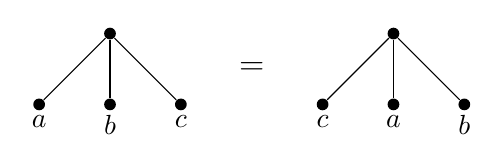
\begin{tikzpicture}[scale=0.9, every node/.style={inner sep=1.5pt}]
    \node (r1) at (0,0) [circle,fill,minimum size=4pt] {};
    \node (a1) at (-1,-1) [circle,fill,minimum size=4pt,label=below:$a$] {};
    \node (b1) at (0,-1) [circle,fill,minimum size=4pt,label=below:$b$] {};
    \node (c1) at (1,-1) [circle,fill,minimum size=4pt,label=below:$c$] {};
    \draw (r1) -- (a1);
    \draw (r1) -- (b1);
    \draw (r1) -- (c1);

    \node at (2, -0.5) {\large $=$};

    \node (r2) at (4,0) [circle,fill,minimum size=4pt] {};
    \node (c2) at (3,-1) [circle,fill,minimum size=4pt,label=below:$c$] {};
    \node (a2) at (4,-1) [circle,fill,minimum size=4pt,label=below:$a$] {};
    \node (b2) at (5,-1) [circle,fill,minimum size=4pt,label=below:$b$] {};
    \draw (r2) -- (c2);
    \draw (r2) -- (a2);
    \draw (r2) -- (b2);
  \end{tikzpicture}
  \end{center}
  \note{%
    Timing: 1:00.

    Let me start with the example I want to study.

    A mobile is a countably branching tree whose children are unordered.

    So we have a leaf, a node, and an equation saying that permuting the
    children of a node does not change the element.

    I write \(\mathcal{M}\) for the quotient inductive type we want to
    construct.

    Mobiles are a good test case because they are infinitary, but the
    defining equations are still very simple.
  }
\end{frame}

% ---------------------------------------------------------------------------
% Slide 4: Naive quotient attempt
% ---------------------------------------------------------------------------
\begin{frame}{Why not quotient a W-type?}
  Let \(W\) be the raw \(W\)-type of ordered countably branching trees.

  \[
    \ell_W : W,
    \qquad
    n_W : (\mathbb N \to W) \to W
  \]

  Form the naive quotient
  \[
    Q := W/{\sim}.
    \qquad\text{Does }Q\text{ carry the right constructor structure?}
  \]
  \note{%
    Timing: 0:45.

    The obvious thing to try is to start with the raw ordered tree type
    \(W\), quotient by permutation, and hope that this quotient is the
    mobile type.

    So \(W\) is the raw tree type, \(Q\) is the naive quotient, and
    \(\mathcal{M}\) is the quotient inductive type we actually want.

    \(Q\) looks to have the right shape element-wise.

    But the problem is whether \(Q\) carries the right constructor
    structure.
  }
\end{frame}

% ---------------------------------------------------------------------------
% Slide 5: The lifting problem
% ---------------------------------------------------------------------------
\begin{frame}[fragile]{The lifting problem}
  The leaf lifts immediately:
  \[
    \widetilde{\ell} := [\ell_W].
  \]

  But for the node we want
  \[
    \widetilde{n} : Q^{\mathbb N} \to Q
  \]
  and the obvious route is blocked:
  \[
  \begin{tikzcd}
      Q^{\mathbb N}
        \arrow[d, dashed, "?"']
        \arrow[rr, dashed, "\widetilde{n}"] &&
      Q \\
      W^{\mathbb N} \arrow[r, "n_W"'] &
      W \arrow[ur, "{[-]_\sim}"']
    \end{tikzcd}
  \]

  To define \(\widetilde{n}\), we would need representatives in \(W\)
  for quotient elements in \(Q\).
  \note{%
    Timing: 2:00.

    This is the central obstruction.

    The leaf is easy. We just take the equivalence class of the raw leaf.

    But the node is different.

    Its input is now a family of quotient elements, not a family of raw
    trees.

    To apply the raw constructor \(n_W\), we would need to choose a
    representative tree for each input.

    Then we could apply \(n_W\) in \(W\), and quotient again.

    This is easy in the finite case, because we can make finitely many
    choices one by one.

    For an infinitary constructor, however, choosing a representative for
    every input is exactly the shape of a choice problem.

    A quotient gives classes, but a constructor wants representatives.

    That representative-picking step is exactly where the problem lives.
  }
\end{frame}


% ---------------------------------------------------------------------------
% Slide 6: The FPS construction
% ---------------------------------------------------------------------------
\begin{frame}{The FPS construction}
  \begin{columns}[T]
    \begin{column}{0.55\textwidth}
      Fiore, Pitts, and Steenkamp (FPS) construct infinitary QITs stagewise.

      \begin{enumerate}
        \item build depth-bounded approximations \(D_\alpha\)
        \item quotient each stage
        \item take \(Q := \mathrm{colim}\,D\)
      \end{enumerate}
      \medskip
    \end{column}
    \begin{column}{0.45\textwidth}
      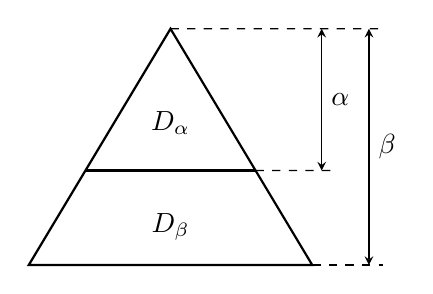
\begin{tikzpicture}[scale=0.6, thick, text=black, draw=black]

        % Define the main vertices
        \coordinate (Top) at (0, 5);
        \coordinate (BottomLeft) at (-3, 0);
        \coordinate (BottomRight) at (3, 0);

        % Draw the main outer triangle (D_\beta boundary)
        \draw (BottomLeft) -- (BottomRight) -- (Top) -- cycle;

        % Define and draw the horizontal subdivision line
        % This partitions the triangle at y=2
        \coordinate (MidLeft) at (-1.8, 2);
        \coordinate (MidRight) at (1.8, 2);
        \draw (MidLeft) -- (MidRight);

        % Place the labels inside their respective regions
        \node at (0, 3) {$D_\alpha$};
        \node at (0, 0.8) {$D_\beta$};

        % Draw thin, dashed guide lines for the vertical dimensions
        \draw[dashed, thin] (Top) -- (4.5, 5);
        \draw[dashed, thin] (MidRight) -- (3.5, 2);
        \draw[dashed, thin] (BottomRight) -- (4.5, 0);

        % Add the vertical dimension arrows and corresponding labels
        \draw[<->, >=stealth, thin] (3.2, 2) -- node[right] {$\alpha$} (3.2, 5);
        \draw[<->, >=stealth, thin] (4.2, 0) -- node[right] {$\beta$} (4.2, 5);

      \end{tikzpicture}
    \end{column}
  \end{columns}

  \vspace{0.5em}

  Weak choice (IWISC) is used at the cocontinuity step:

  \[
    (\mathbb{N} \to \mathrm{colim}\,D) \cong \mathrm{colim}(D^{\mathbb{N}})
  \]

  \note{%
    Timing: 1:15.

    There is already a general answer to this problem, due to Fiore, Pitts,
    and Steenkamp.

    Their idea is to build the quotient inductive type stage by stage.

    First they build bounded approximations, then quotient at each stage,
    and finally take a colimit.

    The hard step is cocontinuity.

    Roughly, cocontinuity says that forming constructor inputs behaves well
    with this colimit.

    That is exactly where weak choice enters their proof.
  }
\end{frame}

% ---------------------------------------------------------------------------
% Slide 7: The question
% ---------------------------------------------------------------------------
\begin{frame}{An observation from mobiles}
  \textbf{Observation}
  \begin{itemize}
    \item permutation equations preserve depth
    \item so equal trees should have the same stage
  \end{itemize}

  \medskip

  \textbf{Obstacle}
  \begin{itemize}
    \item raw tree ordinals still remember the order of children
  \end{itemize}

  \medskip

  \textbf{Question}
  \begin{itemize}
    \item can we replace them by an extensional ordinal basis?
  \end{itemize}

  \note{%
    Timing: 0:45.

    Now mobiles have a special feature.

    Permuting the children of a node does not change their depth, it only
    changes their order.

    So the permutation equations preserve depth.

    That suggests that stage assignment ought to respect the quotient.

    The obstacle is that raw tree ordinals still remember the order of the
    children, so they are not extensional enough for this purpose.

    That leads to the question: can we replace them by an extensional
    ordinal basis?
  }
\end{frame}

% ---------------------------------------------------------------------------
% Slide 8: What we postulate
% ---------------------------------------------------------------------------
\begin{frame}{Extensional plump ordinals}
  Assume an extensional plump ordinal basis for the given signature.
  \[
    \mathsf{sup} : \sum_{s:S} (P_s \to Z) \to Z
  \]

  \medskip

  along with \(\le,<\), such that:

  \[
    \dfrac{\forall i:P_s.\; \xi_i < \alpha}{\mathsf{sup}_s\, \xi \le \alpha}
    \qquad\qquad
    \dfrac{\exists i:P_s.\; \alpha \le \xi_i}{\alpha < \mathsf{sup}_s\, \xi}
  \]

  with extensionality:
  \[
  \dfrac{\forall \gamma.\;(\gamma<\alpha \Leftrightarrow \gamma<\beta)}{\alpha=\beta}
  \]
  \note{%
    Timing: 1:15.

    At this point I need to say clearly what extra structure I am assuming.

    I am not assuming full choice.

    What I postulate is an extensional plump ordinal object \(Z\), equipped
    with a sup constructor for the given signature, together with the order
    structure needed to run the stage argument.

    Crucially, extensionality says that each ordinal is determined by its
    set of strictly smaller ordinals.

    The point is that the stage object itself is now built in a way that
    already respects the relevant identifications.

    This is the extra structure that replaces the choice step in the mobile
    case.
  }
\end{frame}

% ---------------------------------------------------------------------------
% Slide 9: Why extensional ordinals?
% ---------------------------------------------------------------------------
\begin{frame}{Why extensionality is needed}
  Raw plump ordinals still remember the order of children.

  \medskip

  For congruent trees such as
  \[
    n(a,b,c)
    \qquad\text{and}\qquad
    n(b,a,c)
  \]
  the associated raw ordinals \(\alpha\) and \(\beta\) may satisfy
  \[
    \alpha \leq \beta
    \qquad\text{and}\qquad
    \beta \leq \alpha
  \]
  without being literally equal.

  \medskip

  So raw stage assignment does not descend directly.
  It must pass through an extensional quotient.
  \note{%
    Timing: 1:10.

    This is why extensionality is needed, not just raw plump ordinals.

    A raw plump ordinal still remembers the order of the children.

    So if I permute the children, I can get two ordinals that are mutually
    below each other, but not literally equal.

    That is acceptable intensionally, but it is not good enough if stage
    assignment is supposed to respect the quotient.

    So raw stage assignment does not descend directly.

    It has to pass through an extensional quotient of those ordinals.
  }
\end{frame}

% ---------------------------------------------------------------------------
% Slide 10: Proof sketch
% ---------------------------------------------------------------------------
\begin{frame}{Proof sketch}
  For mobiles, permutation equations are depth-preserving.

  \medskip

  So the raw stage assignment
  \[
    d_0 : W \to Z
  \]
  respects the quotient relation at each stage, and descends to maps
  \[
    d_\alpha : D_\alpha \to Z.
  \]

  \medskip

  These descended maps are compatible with the cocone maps, so they
  assemble into
  \[
    d : \mathrm{colim}\,D \to Z.
  \]

  \medskip

  This coherent stage assignment gives the section needed to define the
  constructors on the colimit.

  \note{%
    Timing: 1:45.

    Here is the proof idea.

    First, for mobiles, permutation does not change depth, so the raw stage
    assignment \(d_0 : W \to Z\) respects the quotient relation inside each
    stage.

    That means it descends to maps \(d_\alpha : D_\alpha \to Z\).

    Second, these descended maps are compatible with the connecting maps of
    the diagram, so they induce a single map
    \(d : \mathrm{colim}\,D \to Z\).

    This gives exactly the stable stage assignment needed to define the
    constructors on the colimit.

    So in the mobile case, the cocontinuity argument can be recovered from
    the extensional ordinal basis.
  }
\end{frame}

% ---------------------------------------------------------------------------
% Slide 11: Result for mobiles
% ---------------------------------------------------------------------------
\begin{frame}{Result for mobiles}
  For mobiles, the FPS colimit construction can be carried out relative to
  an extensional plump ordinal basis.

  \medskip

  So in this case, the quotient inductive type of mobiles is obtained
  from the stagewise argument from this basis, without relying on IWISC.
  \medskip
  This argument has been paritally formalized in Agda.
  \note{%
    Timing: 0:30.

    This is the payoff.

    For mobiles, depth preservation gives enough control to recover the
    stagewise construction from the extensional ordinal basis.

    So in this case, the full weak-choice argument is not needed in the same
    way as in the general FPS proof.

    This has also been partially formalised in Agda.
  }
\end{frame}

% ---------------------------------------------------------------------------
% Slide 12: Syntactic criteria
% ---------------------------------------------------------------------------
\begin{frame}{Can we generalise beyond mobiles?}
  The positive case for mobiles comes from a \textbf{syntactic} property:

  \medskip

  \textbf{Depth-preserving equations}
  \begin{quote}
    variables occur at the same depth on both sides
  \end{quote}

  \medskip

  A tempting weakening is some boundedness condition, for example:
  \begin{itemize}
    \item bounded depth shift
    \item \(\alpha\)-locality: both sides have depth \(< \alpha\)
  \end{itemize}

  \medskip

  But this cannot be the whole story:
  \begin{itemize}
    \item a large enough extensional ordinal bound may itself not be
          constructively available
    \item bounded syntax alone does not control ordinal strength in general
  \end{itemize}

  \medskip

  Blass's 1983 example already shows a genuine barrier.
  \note{%
    Timing: 2:00.

    The reason this is interesting is that depth preservation is a purely
    syntactic property.

    You can read it off directly from the equations.

    So the obvious next question is whether one can weaken it.

    The most natural weakenings are bounded depth shift, or locality, where
    both sides of an equation stay below some fixed depth bound.

    But I do not want to oversell that.

    First, even if such a syntactic bound exists, the extensional ordinal
    needed to contain all derived witnesses may itself fail to be
    constructively available.

    And that is exactly the kind of choice-like strength we are trying to
    avoid.

    Second, boundedness on its own does not control ordinal strength in
    general.

    Blass's example, later reframed by Lumsdaine and Shulman, shows that
    even apparently controlled equations can still generate large ordinal
    strength.

    So depth preservation gives a genuine positive case, but the right
    general criterion is still open.
  }
\end{frame}

% ---------------------------------------------------------------------------
% Slide 13: Conclusion
% ---------------------------------------------------------------------------
\begin{frame}{Conclusion}
  \begin{itemize}
    \item Known general constructions of infinitary QITs use weak choice.
    \item For mobiles, depth-preservation lets us recover a stable stage
          assignment.
    \item Extensional plump ordinals provide the ordinal basis for the
          mobile case.
    \item But bounded syntactic criteria alone do not yet explain the
          general case: Blass and Lumsdaine--Shulman show a genuine barrier.
  \end{itemize}

  \medskip

  The open problem is to identify which structural features of equations
  control the need for large ordinal strength or choice principles.
  \note{%
    Timing: 0:45.

    So to conclude: weak choice is not the whole story.

    In depth-preserving examples such as mobiles, equality stays in the same
    stage, and that lets us recover a stable stage assignment.

    Extensional plump ordinals provide the ordinal basis for that positive
    case.

    But this does not yet explain the general infinitary situation.

    The open problem is to identify which structural features of the
    equations control the need for large ordinal strength or choice.
  }
\end{frame}

\begin{frame}
  \centering
  \vfill
  {\LARGE Thank you for listening}
  \vspace{1em}

  Questions?
  \vfill
  \note{%
    Timing: 0:10.
  }
\end{frame}

\begin{frame}[allowframebreaks]{References}
  \tiny
  \begin{thebibliography}{3}

  \bibitem{abbott2005-containers}
  Michael Abbott, Thorsten Altenkirch, and Neil Ghani.
  \newblock Containers: Constructing strictly positive types.
  \newblock {\em Theoretical Computer Science}, 342(1):3--27, 2005.

  \bibitem{altenkirch2016-qit}
  Thorsten Altenkirch and Ambrus Kaposi.
  \newblock Type theory in type theory using quotient inductive types.
  \newblock In {\em Proceedings of the 43rd ACM SIGPLAN-SIGACT Symposium on
    Principles of Programming Languages (POPL 2016)}, pages 18--29, 2016.

  \bibitem{altenkirch2018-qiit}
  Thorsten Altenkirch, Paolo Capriotti, Gabe Dijkstra, Nicolai Kraus, and
  Fredrik Nordvall Forsberg.
  \newblock Quotient inductive-inductive types.
  \newblock In {\em Foundations of Software Science and Computation Structures
    (FoSSaCS 2018)}, pages 293--310, 2018.

  \bibitem{altenkirch2017-partiality-monad}
  Thorsten Altenkirch, Nils Anders Danielsson, and Nicolai Kraus.
  \newblock Partiality, revisited: The partiality monad as a quotient inductive-inductive type.
  \newblock In {\em Foundations of Software Science and Computation Structures (FoSSaCS 2017)}, pages 17--33, 2017.

  \bibitem{fiore2022-quotients-inductive-types}
  Marcelo P.~Fiore, Andrew M.~Pitts, and S.~C.~Steenkamp.
  \newblock Quotients, inductive types, and quotient inductive types.
  \newblock {\em Logical Methods in Computer Science}, 18(2), 2022.

  \bibitem{kaposi2019-constructing}
  Ambrus Kaposi, Andr\'as Kov\'acs, and Thorsten Altenkirch.
  \newblock Constructing quotient inductive-inductive types.
  \newblock {\em Proceedings of the ACM on Programming Languages},
    3(POPL):2:1--2:24, 2019.

  \bibitem{kaposi2021-setoid}
  Ambrus Kaposi and Zongpu Xie.
  \newblock Quotient inductive-inductive types in the setoid model.
  \newblock In {\em 27th International Conference on Types for Proofs and
    Programs (TYPES 2021)}, presentation abstract/slides, 2021.

  \bibitem{kovacs2020-large}
  Andr\'as Kov\'acs and Ambrus Kaposi.
  \newblock Large and infinitary quotient inductive-inductive types.
  \newblock In {\em Proceedings of the 35th Annual ACM/IEEE Symposium on Logic in
    Computer Science (LICS 2020)}, pages 648--661, 2020.

  \bibitem{kraus2023-ordinal}
  Nicolai Kraus, Fredrik Nordvall Forsberg, and Chuangjie Xu.
  \newblock Type-theoretic approaches to ordinals.
  \newblock {\em Theoretical Computer Science}, 957:113843, 2023.

  \bibitem{lumsdaine2020-hit}
  Peter LeFanu Lumsdaine and Michael Shulman.
  \newblock Semantics of higher inductive types.
  \newblock {\em Mathematical Proceedings of the Cambridge Philosophical
    Society}, 169(1):159--208, 2020.

  \bibitem{taylor1996-intuitionistic}
  Paul Taylor.
  \newblock Intuitionistic sets and ordinals.
  \newblock {\em The Journal of Symbolic Logic}, 61(3):705--744, 1996.

  \bibitem{taylor1999-practical}
  Paul Taylor.
  \newblock Practical Foundations of Mathematics.
  \newblock {\em Cambridge Studies in Advanced Mathematics}, volume 59. Cambridge University Press, 1999.

  \bibitem{hott2013-book}
  The Univalent Foundations Program.
  \newblock Homotopy Type Theory: Univalent Foundations of Mathematics.
  \newblock Institute for Advanced Study, 2013.

  \bibitem{vandenberg2012-wisc-axiom}
  Benno van den Berg and Ieke Moerdijk.
  \newblock The axiom of multiple choice and models for constructive set theory.
  \newblock {\em arXiv preprint arXiv:1204.4045}, 2012.

  \end{thebibliography}
\end{frame}

\end{document}

